% ----------------------------------------------------------
\chapter{HISTÓRIAS DE USUÁRIO}
% ----------------------------------------------------------

\begin{itemize}
    \item HU01 Cadastro do Usuário
    \item HU02 Realizar Login/Logout
    \item HU03 Criar Boletos
    \item HU04 Deletar Boletos
    \item HU05 Editar Boletos
    \item HU06 Criar fonte de Renda
    \item HU07 Deletar fonte de Renda
    \item HU08 Editar fonte de Renda
    \item HU09 Criar Orçamento
    \item HU10 Deletar Orçamento
    \item HU11 Editar Orçamento
    \item HU12 Visualizar Resumo

\end{itemize}

\section{Detalhamento das histórias}

\subsection{HU01 Cadastro do Usuário}

Sendo um novo usuario da aplicação, quero me cadastrar na aplicacao, para que consiga usar a aplicação com segurança.

\begin{figure}[htb]
	\caption{\label{fig:hu01}Cadastro de usuário.}
	\begin{center}
		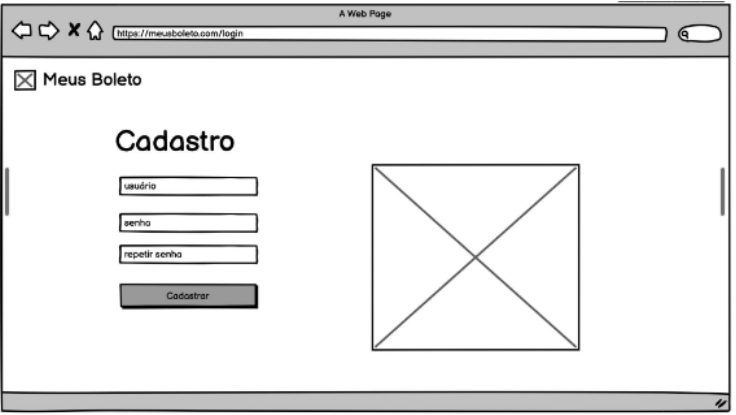
\includegraphics[scale=0.5]{images/Cadastro.png}
	\end{center}
	\fonte{Autor (2024)}
\end{figure}

\textbf{CRITÉRIOS DE ACEITAÇÃO}

\begin{enumerate}
    \item Deve permitir o usuário cadastrar no sistema informando um apelido e senha.
    \item Não deve permitir campos vazios
    \item Não deve permitir senha com menos de 12 caracteres
    \item Deve validar se usuário já existe
    \item Deve validar se as senhas são iguais
\end{enumerate}

\textbf{CRITÉRIOS DE ACEITAÇÃO - DETALHAMENTO}

\textbf{Critério de contexto (Válido como premissa para todos os critérios):}

\begin{itemize}
    \item[\textbf{Dado que}] não tenho acesso a aplicação
    \item[\textbf{E}] estou na tela de cadastro
\end{itemize}


\begin{itemize}
    \item[] \textbf{1. Deve permitir o usuário cadastrar no sistema informando um apelido e senha}

    \begin{itemize}
        \item[\textbf{Dado que}] preenchi o campo senha
        \item[\textbf{E}] o campo do 'repetir senha'.
        \item[\textbf{E}] o campo do usuário.
        \item[\textbf{Quando}] pressiono o botão ``Cadastrar''
        \item[\textbf{Então}] o sistema deve realizar o registro dos meus dados
    \end{itemize}

    \item[] \textbf{2. Não deve permitir campos vazios}
    
    \begin{itemize}
        \item[\textbf{Dado que}] não preenchi algum campo da tela
        \item[\textbf{Quando}] pressiono o botão ``Cadastrar''
        \item[\textbf{Então}] o sistema deve apresentar um erro me informando (R1)
    \end{itemize}

     \item[] \textbf{3. Não deve permitir senha com menos de 12 caracteres}
    
    \begin{itemize}
        \item[\textbf{Dado que}] preenchi o campo da senha com menos de 12 caracteres
        \item[\textbf{E}] e o campo de repetir com a mesma senha
        \item[\textbf{Quando}] pressiono o botão ``Cadastrar''
        \item[\textbf{Então}] o sistema deve apresentar um erro dizendo ao usuário sobre o tamanho das senhas (R1)
    \end{itemize}

     \item[] \textbf{4. Deve validar se usuário já existe}
    
    \begin{itemize}
        \item[\textbf{Dado que}] preenchi o campo de usuário
        \item[\textbf{E}] o campo das senhas corretamente
        \item[\textbf{Quando}] pressiono o botão ``Cadastrar''
        \item[\textbf{Então}] o sistema deve validar se o usuário já existe no sistema se sim, deve apresentar o erro ao usuário (R1)
    \end{itemize}

     \item[] \textbf{5. Deve validar se as senhas são iguais}
    
    \begin{itemize}
        \item[\textbf{Dado que}] preenchi o campo da senha com uma senha
        \item[\textbf{E}] a repetição da senha com outra
        \item[\textbf{Quando}] pressiono o botão ``Cadastrar''
        \item[\textbf{Então}] o sistema deve verificar se as senhas são iguais e aprentar a mensagem de erro apropriada.(R1)
    \end{itemize}

  
\end{itemize}

\textbf{REGRAS DE NEGÓCIO DA HISTÓRIA:}

    R1 - Campos inconsistentes

    \begin{table}[htb]
        \caption{Tabela de inconsistências de cadastro}
        \centering
        \begin{tabular}{|c|c|}
        \hline
          \textbf{Incosistência}   &  \textbf{Mensagem} \\
        \hline
        Campos vazios   & "O campo não deve estar vazio!" \\
        \hline
        Senha não permitida   & "A senha deve possuir 12 ou mais caracteres!" \\
        \hline
        Senhas não conferem   & "As senhas devem ser iguais" \\
        \hline
        \end{tabular}
        \fonte{Autor (2024)}
        \label{tab:tabela_cadastro}
    \end{table}
    
\subsection{HU02 Realizar Login/Logout}

Sendo um usuario da aplicação, quero logar na aplicação para que consiga acessar meus dados.

\begin{figure}[htb]
	\caption{\label{fig:hu02}Login do usuário.}
	\begin{center}
		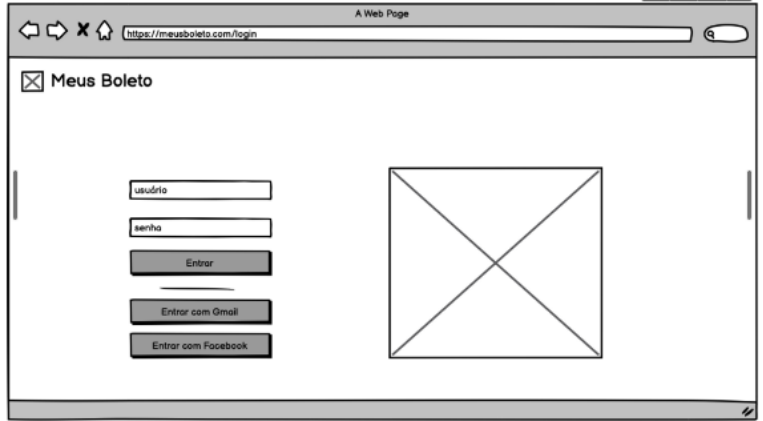
\includegraphics[scale=0.5]{images/Login.png}
	\end{center}
	\fonte{Autor (2024)}
\end{figure}


\textbf{CRITÉRIOS DE ACEITAÇÃO}

\begin{enumerate}
    \item Deve permitir o usuário entrar no sistema.
    \item Deve validar usuário se senha
    \item Não deve permitir acesse se dados estivem incorretos
\end{enumerate}

\textbf{CRITÉRIOS DE ACEITAÇÃO - DETALHAMENTO}

\textbf{Critério de contexto (Válido como premissa para todos os critérios):}

\begin{itemize}
    \item[\textbf{Dado que}] eu tenho um nome de usuário e senha da aplicação
    \item[\textbf{E}] estou na tela de login
\end{itemize}


\begin{itemize}
    \item[] \textbf{1. Deve permitir o usuário entrar no sistema.}

    \begin{itemize}
        \item[\textbf{Dado que}] preenchi o campo 'usuário'
        \item[\textbf{E}] o campo do 'senha'.
        \item[\textbf{Quando}] pressiono o botão ``Entrar''
        \item[\textbf{Então}] o sistema deve permitir a minha estrada no sistema levando-o a tela inicial.
    \end{itemize}

    \item[] \textbf{2. Deve validar usuário se senha.}

    \begin{itemize}
        \item[\textbf{Dado que}] preenchi o campo usuário
        \item[\textbf{E}] o campo 'senha'
        \item[\textbf{Quando}] pressiono o botão ``Entrar''
        \item[\textbf{Então}] o sistema deve realizar validar meus dados
    \end{itemize}

    \item[] \textbf{2. Não deve permitir acesse se dados estivem incorretos.}

    \begin{itemize}
        \item[\textbf{Dado que}] preenchi o campo usuário
        \item[\textbf{Ou}] o campo 'senha' incorretamente
        \item[\textbf{Quando}] pressiono o botão ``Entrar''
        \item[\textbf{Então}] o sistema deve enviar uma mensagem genérica de erro (R2)
    \end{itemize}
\end{itemize}

\textbf{REGRAS DE NEGÓCIO DA HISTÓRIA:}

    R2 - Campos inconsistentes

    \begin{table}[]
        \caption{Tabela de inconsistências de login}
        \centering
        \begin{tabular}{|c|c|}
        \hline
          \textbf{Incosistência}   &  \textbf{Mensagem} \\
        \hline
        Usuário Incorreto   & "Senha ou usuário estão incorretos!" \\
        \hline
        Senha Incorreta   & "Senha ou usuário estão incorretos!" \\
        \hline
        \end{tabular}
        \fonte{Autor (2024)}
        \label{tab:tabela_login}
    \end{table}

\subsection{HU03 Criar Boletos}

Sendo um usuário da aplicação, quero inserir um novo item de despesa/renda para que eu tenha um controle maior de minha dívidas/receitas.

\begin{figure}[h]
	\caption{\label{fig:hu03}Página para criar boletos.}
	\begin{center}
		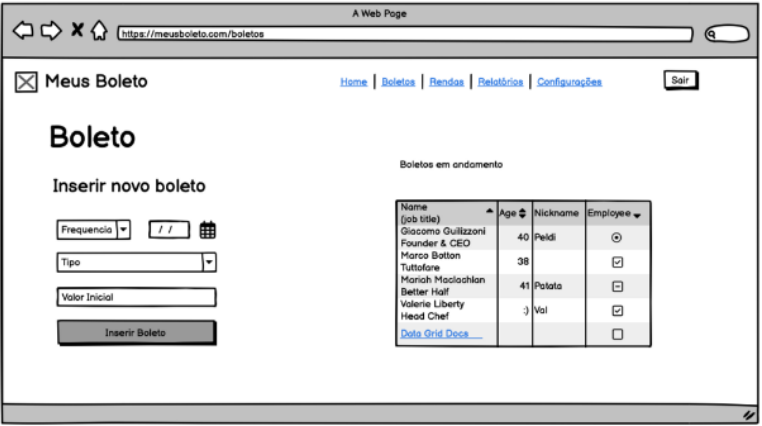
\includegraphics[scale=0.5]{images/CriarBoletoRenda.png}
	\end{center}
	\fonte{Autor (2024)}
\end{figure}


\textbf{CRITÉRIOS DE ACEITAÇÃO}

\begin{enumerate}
    \item Não deve inserir uma data válida;
    \item Deve permitir inserir um novo ‘boleto’ na base de dados para o
usuário;
    \item Deve inserir valores que não sejam números.
\end{enumerate}

\textbf{CRITÉRIOS DE ACEITAÇÃO - DETALHAMENTO}

\textbf{Critério de contexto (Válido como premissa para todos os critérios):}

\begin{itemize}
    \item[\textbf{Dado que}] entrei na aplicação
    \item[\textbf{E}] estou na tela para criacação de boletos
\end{itemize}


\begin{itemize}
    \item[] \textbf{1. Não deve inserir uma data válida;}

    \begin{itemize}
        \item[\textbf{Dado que}] preenchi o campo data com um valor invalido
        \item[\textbf{Quando}] pressiono o botão ``Inserir boleto''
        \item[\textbf{Então}] o sistema deve apresentar uma mensagem de erro avisando a incosistência (R3)
    \end{itemize}

    \item[] \textbf{2. Deve permitir inserir um novo ‘boleto’ na base de dados para o
usuário.}

    \begin{itemize}
        \item[\textbf{Dado que}] preenchi todos os campos corretamente
        \item[\textbf{Quando}] pressiono o botão ``Inserir Boleto''
        \item[\textbf{Então}] o sistema deve realizar a operação e informar o usuario
    \end{itemize}

    \item[] \textbf{3. Não deve permitir valores que não sejam números.}

    \begin{itemize}
        \item[\textbf{Dado que}] preenchi o campo 'Valor Inicial' com caracteres não números
        \item[\textbf{Quando}] pressiono o botão ``Inserir Boleto''
        \item[\textbf{Então}]  o sistema deve apresentar uma mensagem de erro avisando a incosistência (R3)
    \end{itemize}

    
\end{itemize}

\textbf{REGRAS DE NEGÓCIO DA HISTÓRIA:}

    R3 - Campos inconsistentes

    \begin{table}[htb]
        \caption{Tabela de inconsistências de inserir boletos}
        \centering
        \begin{tabular}{|c|c|}
        \hline
          \textbf{Incosistência}   &  \textbf{Mensagem} \\
        \hline
        Valor incorreto   & "O campo de valor somente aceita números!" \\
        \hline
        Data com caracteres inconsistêntes   & "verifique o campo de data!"  \\
        \hline
        \end{tabular}
        \fonte{Autor (2024)}
        \label{tab:tabela_login}
    \end{table}

\subsection{HU04 Deletar Boletos}

Sendo um usuário da aplicação, quero deletar item existente de despesa/renda para que eu exclua ele de minha dívidas/receitas.

\begin{figure}[htb]
	\caption{\label{fig:hu04}Página para deletar boletos.}
	\begin{center}
		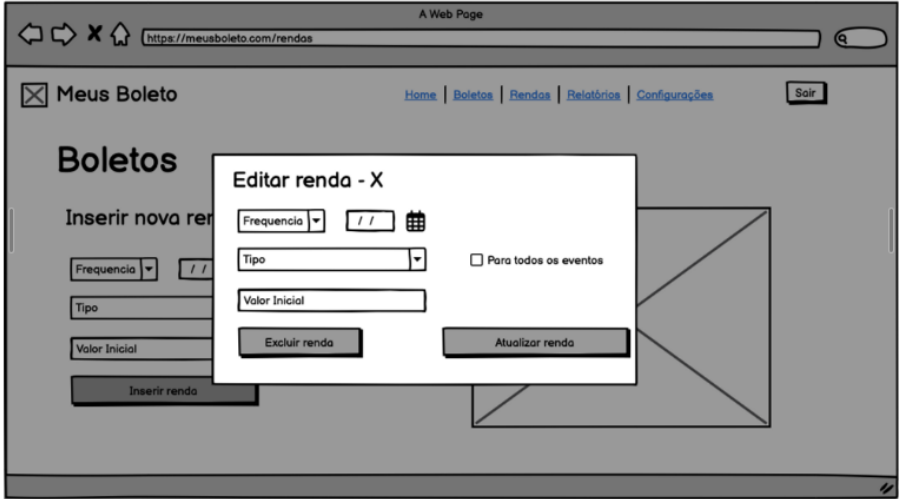
\includegraphics[scale=0.5]{images/EditarBoletoRenda.png}
	\end{center}
	\fonte{Autor (2024)}
\end{figure}

\textbf{CRITÉRIOS DE ACEITAÇÃO}

\begin{enumerate}
    \item Deve permitir o usuário excluir um boleto.
\end{enumerate}

\textbf{CRITÉRIOS DE ACEITAÇÃO - DETALHAMENTO}

\textbf{Critério de contexto (Válido como premissa para todos os critérios):}

\begin{itemize}
    \item[\textbf{Dado que}] entrei na aplicação
    \item[\textbf{E}] estou na tela para seleção de boleto
\end{itemize}


\begin{itemize}
    \item[] \textbf{1. Deve permitir o usuário excluir um boleto.}

    \begin{itemize}
        \item[\textbf{Dado que}] Selecionei um boleto para edição
        \item[\textbf{Quando}] pressiono o botão ``Excluir boleto''
        \item[\textbf{Então}] o sistema deve excluir a transação do sistema
    \end{itemize}
\end{itemize}

\subsection{HU05 Editar Boletos}

Sendo um usuário da aplicação, quero inserir um novo item de despesa/renda para que eu tenha um controle maior de minha dívidas/receitas.

\begin{figure}[htb]
	\caption{\label{fig:hu05}Página para editar boletos.}
	\begin{center}
		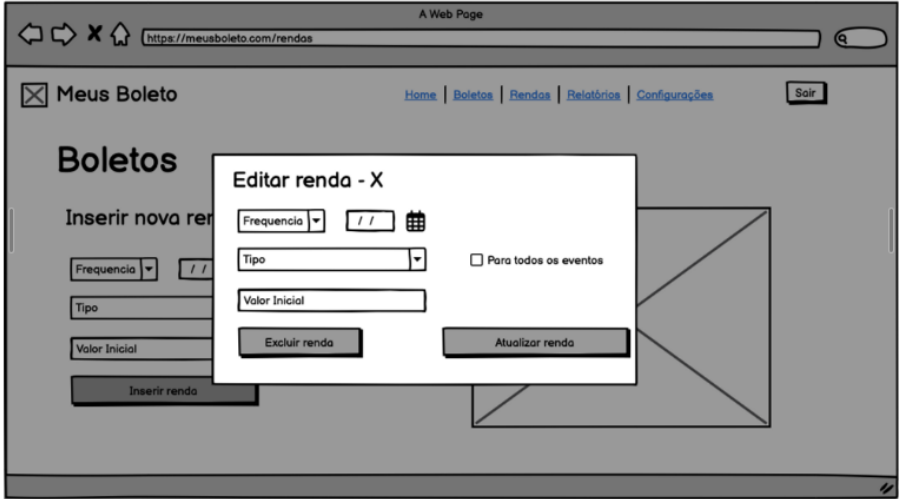
\includegraphics[scale=0.5]{images/EditarBoletoRenda.png}
	\end{center}
	\fonte{Autor (2024)}
\end{figure}


\textbf{CRITÉRIOS DE ACEITAÇÃO}

\begin{enumerate}
    \item Deve permitir a edição de um boleto.
\end{enumerate}

\textbf{CRITÉRIOS DE ACEITAÇÃO - DETALHAMENTO}

\textbf{Critério de contexto (Válido como premissa para todos os critérios):}

\begin{itemize}
    \item[\textbf{Dado que}] entrei na aplicação
    \item[\textbf{E}] estou na tela para seleção de boleto
\end{itemize}


\begin{itemize}
    \item[] \textbf{1. Deve permitir a edição de um boleto.}

    \begin{itemize}
        \item[\textbf{Dado que}] Selecionei um boleto para edição
        \item[\textbf{Quando}] clico em editar
        \item[\textbf{Então}] o sistema deve exibir o modal da figura \ref{fig:hu05} 
    \end{itemize}
\end{itemize}

\subsection{HU06 Criar fonte de Renda}

Sendo um usuário da aplicação, quero editar um item de despesa/renda para que eu consiga atualizar algum valor.

\begin{figure}[htb]
	\caption{\label{fig:hu06}Página para criar fonte de renda.}
	\begin{center}
		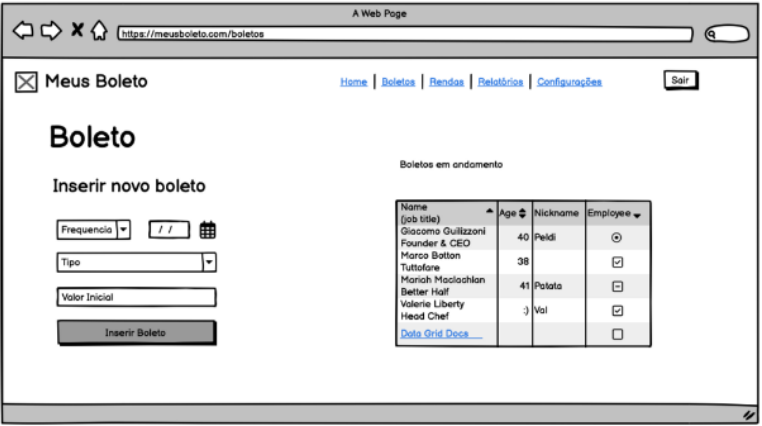
\includegraphics[scale=0.5]{images/CriarBoletoRenda.png}
	\end{center}
	\fonte{Autor (2024)}
\end{figure}

\textbf{CRITÉRIOS DE ACEITAÇÃO}

\begin{enumerate}
    \item Não deve inserir uma data válida;
    \item Deve permitir inserir uma nova ‘Renda’ na base de dados para o
usuário;
    \item Deve inserir valores que não sejam números.
\end{enumerate}

\textbf{CRITÉRIOS DE ACEITAÇÃO - DETALHAMENTO}

\textbf{Critério de contexto (Válido como premissa para todos os critérios):}

\begin{itemize}
    \item[\textbf{Dado que}] entrei na aplicação
    \item[\textbf{E}] estou na tela para criação de rendas
\end{itemize}


\begin{itemize}
    \item[] \textbf{1. Não deve inserir uma data válida;}

    \begin{itemize}
        \item[\textbf{Dado que}] preenchi o campo data com um valor invalido
        \item[\textbf{Quando}] pressiono o botão ``Inserir boleto''
        \item[\textbf{Então}] o sistema deve apresentar uma mensagem de erro avisando a incosistência (R4)
    \end{itemize}

    \item[] \textbf{2. Deve permitir inserir uma nova ‘Renda’ na base de dados para o
usuário.}

    \begin{itemize}
        \item[\textbf{Dado que}] preenchi todos os campos corretamente
        \item[\textbf{Quando}] pressiono o botão ``Inserir Renda''
        \item[\textbf{Então}] o sistema deve realizar a operação e informar o usuário (R4)
    \end{itemize}

    \item[] \textbf{3. Não deve permitir valores que não sejam números.}

    \begin{itemize}
        \item[\textbf{Dado que}] preenchi o campo 'Valor Inicial' com caracteres não números
        \item[\textbf{Quando}] pressiono o botão ``Inserir Boleto''
        \item[\textbf{Então}]  o sistema deve apresentar uma mensagem de erro avisando a inconsistência (R4)
    \end{itemize}

    
\end{itemize}

\textbf{REGRAS DE NEGÓCIO DA HISTÓRIA:}

    R4 - Campos inconsistentes

    \begin{table}[htb]
        \caption{Tabela de inconsistências de inserir rendas}
        \centering
        \begin{tabular}{|c|c|}
        \hline
          \textbf{Incosistência}   &  \textbf{Mensagem} \\
        \hline
        Valor incorreto   & "O campo de valor somente aceita números!" \\
        \hline
        Data com caracteres inconsistêntes   & "verifique o campo de data!"  \\
        \hline
        \end{tabular}
        \fonte{Autor (2024)}
        \label{tab:tabela_renda_inss }
    \end{table}


\subsection{HU07 Deletar fonte de Renda}

Sendo um usuário da aplicação, quero deletar um item de renda para que eu consiga excluir o item selecionado.

\begin{figure}[htb]
	\caption{\label{fig:hu07}Página para deletar fonte de renda.}
	\begin{center}
		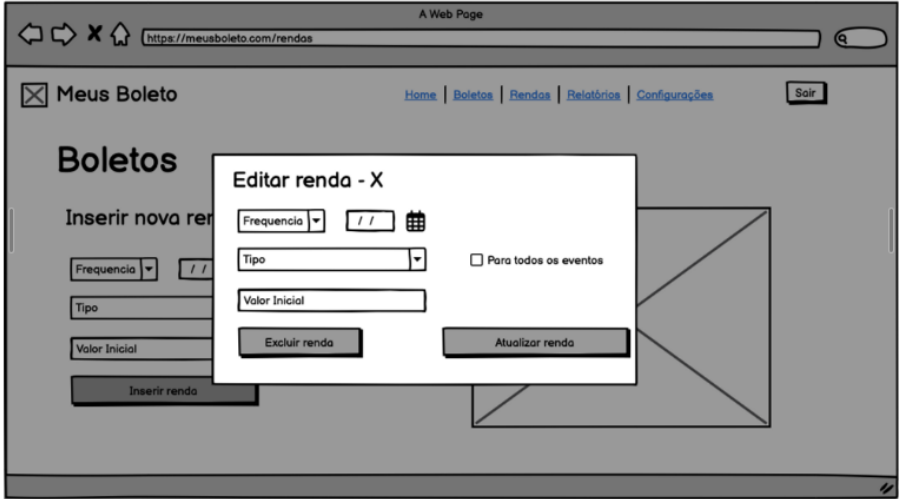
\includegraphics[scale=0.5]{images/EditarBoletoRenda.png}
	\end{center}
	\fonte{Autor (2024)}
\end{figure}

\textbf{CRITÉRIOS DE ACEITAÇÃO}

\begin{enumerate}
    \item Deve permitir o usuário excluir uma renda.
    
\end{enumerate}

\textbf{CRITÉRIOS DE ACEITAÇÃO - DETALHAMENTO}

\textbf{Critério de contexto (Válido como premissa para todos os critérios):}

\begin{itemize}
    \item[\textbf{Dado que}] entrei na aplicação
    \item[\textbf{E}] estou na tela para seleção de renda
\end{itemize}


\begin{itemize}
    \item[] \textbf{1. Deve permitir o usuário excluir uma fonte de renda.}

    \begin{itemize}
        \item[\textbf{Dado que}] Selecionei uma renda para edição
        \item[\textbf{Quando}] pressiono o botão ``Excluir Renda''
        \item[\textbf{Então}] o sistema deve excluir a transação do sistema
    \end{itemize}
\end{itemize}


\subsection{HU08 Editar fonte de Renda}

Sendo um usuário da aplicação, quero editar um item de renda para que eu consiga atualizar o item selecionado.

\begin{figure}[htb]
	\caption{\label{fig:hu07}Página para editar fonte de renda.}
	\begin{center}
		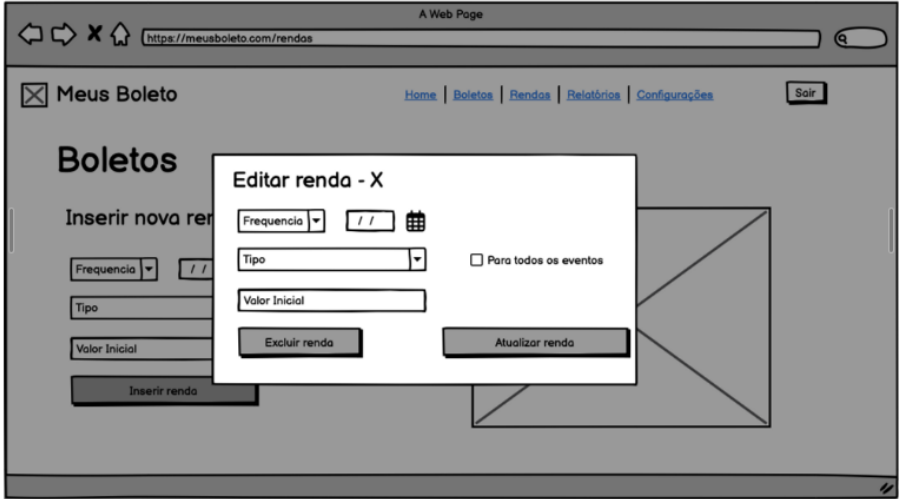
\includegraphics[scale=0.5]{images/EditarBoletoRenda.png}
	\end{center}
	\fonte{Autor (2024)}
\end{figure}

\textbf{CRITÉRIOS DE ACEITAÇÃO}

\begin{enumerate}
    \item Deve permitir a edição de uma renda.
\end{enumerate}

\textbf{CRITÉRIOS DE ACEITAÇÃO - DETALHAMENTO}

\textbf{Critério de contexto (Válido como premissa para todos os critérios):}

\begin{itemize}
    \item[\textbf{Dado que}] entrei na aplicação
    \item[\textbf{E}] estou na tela para seleção de renda
\end{itemize}


\begin{itemize}
    \item[] \textbf{1. Deve permitir a edição de uma renda.}

    \begin{itemize}
        \item[\textbf{Dado que}] Selecionei uma renda para edição
        \item[\textbf{Quando}] clico em editar
        \item[\textbf{Então}] o sistema deve exibir o modal da figura \ref{fig:hu07} 
    \end{itemize}
\end{itemize}

\subsection{HU12 Visualizar Resumo}

Sendo um usuário da aplicação, quero visualizar um resumo logo que entrar na aplicação para que eu veja os próximos vencimentos e créditos.

\begin{figure}[htb]
	\caption{\label{fig:Fig_1}Página inicial da aplicação.}
	\begin{center}
		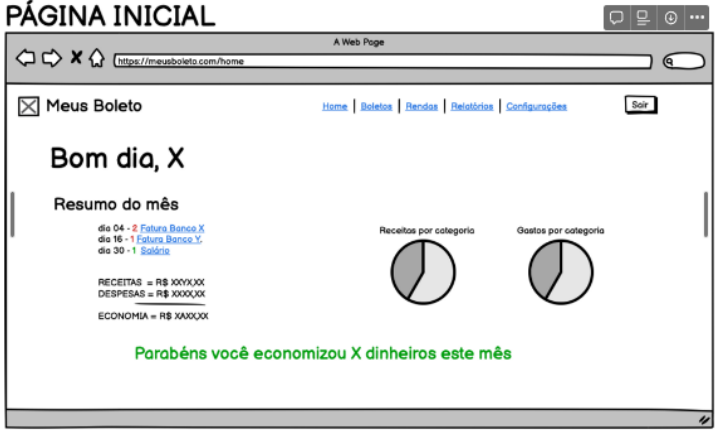
\includegraphics[scale=0.5]{images/TelaInicial.png}
	\end{center}
	\fonte{Autor (2024)}
\end{figure}

\textbf{CRITÉRIOS DE ACEITAÇÃO}

\begin{enumerate}
    \item Deve mostrar um gráfico resumindo as despesas do mês.
    \item Deve mostrar um resumo do saldo final.
\end{enumerate}

\textbf{CRITÉRIOS DE ACEITAÇÃO - DETALHAMENTO}

\textbf{Critério de contexto (Válido como premissa para todos os critérios):}

\begin{itemize}
    \item[\textbf{Dado que}] entrei na aplicação
    \item[\textbf{E}] estou na tela para seleção de renda
\end{itemize}


\begin{itemize}

      \item[] \textbf{1. Deve mostrar um gráfico resumindo as despesas do mês.}

    \begin{itemize}
        \item[\textbf{Dado que}] Estou na página inicial
        \item[\textbf{Então}] o sistema deve exibir o gráficos de resumo mensal de pr \ref{fig:hu07} 
    \end{itemize}

    \item[] \textbf{2. Deve mostrar um resumo do saldo final.}

    \begin{itemize}
        \item[\textbf{Dado que}]  Estou na página inicial
        \item[\textbf{Então}] o sistema deve exibir o resumo mensal das contas 
    \end{itemize}
    
\end{itemize}